\documentclass[11pt]{article}
\usepackage{amsmath, amssymb, physics, mathtools, bm}
\usepackage{tikz, pgfplots}
\pgfplotsset{compat=1.18}
\usetikzlibrary{decorations.markings, decorations.pathmorphing, arrows.meta, positioning}
\tikzset{
  ->-/.style={
    decoration={markings, mark=at position #1 with {\arrow{>}}},
    postaction={decorate}
  },
  ->-/.default=0.55
}
\usepackage[margin=2.3cm]{geometry}
\usepackage{siunitx, booktabs, hyperref}
\usepackage{braket}

\newcommand{\D}{\mathrm{D}}
\newcommand{\de}{\mathrm{d}}
\newcommand{\pd}[2]{\frac{\partial #1}{\partial #2}}
\newcommand{\Lap}{\nabla^{2}}
\newcommand{\Kz}{K^{0}}
\newcommand{\Kbar}{\overline{K^{0}}}

\title{B4 Nuclear and Particle Physics --- Model Solutions, Trinity 2022}
\author{}
\date{}

\begin{document}
\maketitle

%==========================================================
\section*{Question 1 --- Neutral kaon mixing and oscillation}

\textbf{Problem.} (a) Leading-order $\Kz \leftrightarrow \Kbar$ mixing diagram. (b) From $|\pm\rangle = \tfrac{1}{\sqrt2}(|\Kz\rangle\pm|\Kbar\rangle)$ being $CP$-eigenstates, deduce $C$, the pion content of each decay, draw diagrams, and explain $\tau_S\ll\tau_L$. (c) Threshold for $pp\to p\pi^+\Lambda^0\Kz$, quark-flow diagram, regeneration. (d) Justify $A_S(t)=A_S(0)e^{-im_St}e^{-t/(2\tau_S)}$ and write $A_{\Kz},A_{\Kbar}$. (e) For initial pure $\Kz$, find $A,B,C,\phi$ and sketch.

\subsection*{(a)}

$\Kz=(d\bar s)$, $\Kbar=(\bar d s)$: $|\Delta S|=2$ requires second-order weak box diagram with internal $u,c,t$.

\begin{center}
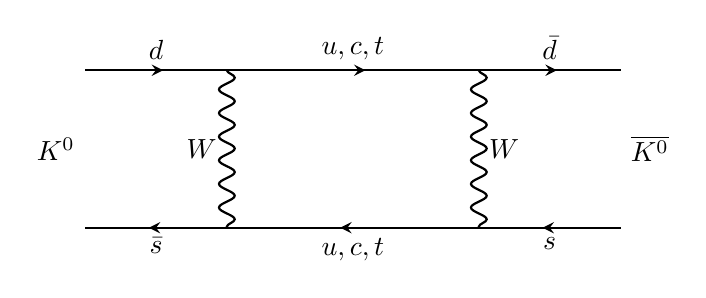
\begin{tikzpicture}[thick, scale=1.0, >=stealth]
  \draw[->-] (-3.4,1.0) -- (-1.6,1.0) node[midway,above]{$d$};
  \draw[->-] (-1.6,-1.0) -- (-3.4,-1.0) node[midway,below]{$\bar s$};
  \draw[->-] (1.6,1.0) -- (3.4,1.0) node[midway,above]{$\bar d$};
  \draw[->-] (3.4,-1.0) -- (1.6,-1.0) node[midway,below]{$s$};
  \draw[->-] (-1.6,1.0) -- (1.6,1.0) node[midway,above]{$u,c,t$};
  \draw[->-] (1.6,-1.0) -- (-1.6,-1.0) node[midway,below]{$u,c,t$};
  \draw[decorate, decoration={snake, amplitude=1mm, segment length=3mm}] (-1.6,1.0) -- (-1.6,-1.0) node[midway,left]{$W$};
  \draw[decorate, decoration={snake, amplitude=1mm, segment length=3mm}] (1.6,1.0) -- (1.6,-1.0) node[midway,right]{$W$};
  \node[left] at (-3.4,0) {$\Kz$};
  \node[right] at (3.4,0) {$\Kbar$};
\end{tikzpicture}
\end{center}

\subsection*{(b)}

$CP$ eigenvalues by hypothesis:
\[ CP|+\rangle = +|+\rangle,\qquad CP|-\rangle = -|-\rangle. \]
Substitute the $|\pm\rangle$ definitions:
\[ CP|\Kz\rangle = -|\Kbar\rangle,\qquad CP|\Kbar\rangle = -|\Kz\rangle. \]
Use $P|\Kz\rangle = -|\Kz\rangle$ (pseudoscalar):
\[ \boxed{\;C|\Kz\rangle = +|\Kbar\rangle,\qquad C|\Kbar\rangle = +|\Kz\rangle.\;} \]

\textbf{Pion content.} For $J=0$ kaons, $CP(n\pi)=(-1)^n$:
\[ |+\rangle\;(CP=+1)\to 2\pi,\qquad |-\rangle\;(CP=-1)\to 3\pi. \]

\begin{center}
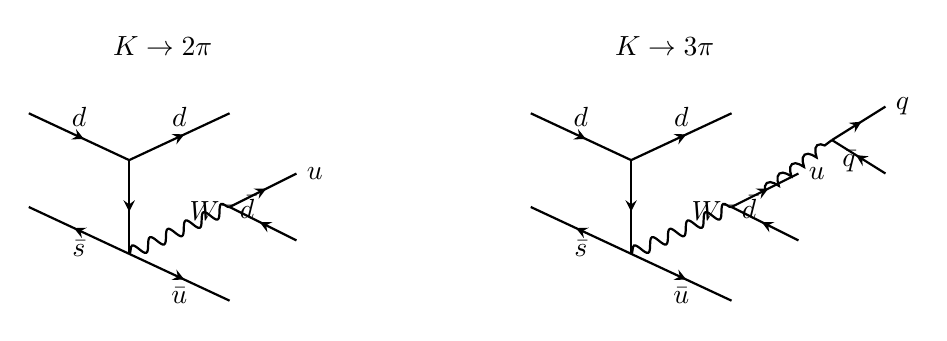
\begin{tikzpicture}[thick, scale=0.85, >=stealth]
  \node at (-4.5,2.4) {\textbf{$K\to 2\pi$}};
  \draw[->-] (-6.5,1.4) -- (-5,0.7) node[midway,above]{$d$};
  \draw[->-] (-5,0.7) -- (-3.5,1.4) node[midway,above]{$d$};
  \draw[->-] (-5,-0.7) -- (-6.5,-0.0) node[midway,below]{$\bar s$};
  \draw[->-] (-5,-0.7) -- (-3.5,-1.4) node[midway,below]{$\bar u$};
  \draw[->-] (-5,0.7) -- (-5,-0.7);
  \node[left] at (-5.0,0) {};
  \draw[decorate, decoration={snake, amplitude=0.8mm, segment length=2.5mm}] (-5,-0.7) -- (-3.5,0) node[midway,above right]{$W^-$};
  \draw[->-] (-3.5,0) -- (-2.5,0.5) node[right]{$u$};
  \draw[->-] (-2.5,-0.5) -- (-3.5,0) node[right]{$\bar d$};
  %
  \node at (3,2.4) {\textbf{$K\to 3\pi$}};
  \draw[->-] (1,1.4) -- (2.5,0.7) node[midway,above]{$d$};
  \draw[->-] (2.5,0.7) -- (4,1.4) node[midway,above]{$d$};
  \draw[->-] (2.5,-0.7) -- (1,0) node[midway,below]{$\bar s$};
  \draw[->-] (2.5,-0.7) -- (4,-1.4) node[midway,below]{$\bar u$};
  \draw[->-] (2.5,0.7) -- (2.5,-0.7);
  \draw[decorate, decoration={snake, amplitude=0.8mm, segment length=2.5mm}] (2.5,-0.7) -- (4,0) node[midway,above right]{$W^-$};
  \draw[->-] (4,0) -- (5,0.5) node[right]{$u$};
  \draw[->-] (5,-0.5) -- (4,0) node[right]{$\bar d$};
  \draw[decorate, decoration={coil, aspect=0.4, segment length=2mm, amplitude=0.6mm}] (4.5,0.25) -- (5.5,1.0);
  \draw[->-] (5.5,1.0) -- (6.3,1.5) node[right]{$q$};
  \draw[->-] (6.3,0.5) -- (5.5,1.0) node[below right]{$\bar q$};
\end{tikzpicture}
\end{center}

\textbf{Lifetime ordering.} $Q$-values:
\[ Q_{2\pi} = m_K - 2 m_\pi \approx 220\text{ MeV},\qquad Q_{3\pi} = m_K - 3 m_\pi \approx 80\text{ MeV}. \]
Phase space drives $\Gamma$, so:
\[ \boxed{\;K^0_S \leftrightarrow |+\rangle\to 2\pi,\qquad K^0_L\leftrightarrow|-\rangle\to 3\pi,\qquad \tau_L/\tau_S\sim 580.\;} \]

\subsection*{(c)}

\textbf{Threshold.} Mandelstam $s$ at threshold (all final-state particles at rest in c.m.):
\[ \sqrt{s}_{\min} = m_p + m_{\pi^+} + m_\Lambda + m_{\Kz} \equiv M. \]
Lab frame, target proton at rest:
\[ s = 2 m_p E_1 + 2 m_p^2. \]
Equate:
\[ 2 m_p E_{1,\min} + 2 m_p^2 = M^2. \]
Solve for $E_{1,\min}$:
\[ \boxed{\;E_{1,\min} = \frac{M^2 - 2 m_p^2}{2 m_p},\qquad T_{1,\min} = E_{1,\min} - m_p.\;} \]
Numerical: $M = 938.3 + 139.6 + 1115.7 + 497.6 = 2691.2$ MeV/$c^2$:
\[ M^2 = 7.242\times 10^{6}\text{ MeV}^2,\qquad 2m_p^2 = 1.761\times 10^{6}\text{ MeV}^2. \]
\[ E_{1,\min} = \frac{7.242\times 10^6 - 1.761\times 10^6}{2\times 938.3}\text{ MeV} = 2920\text{ MeV}. \]
\[ T_{1,\min} \approx 1.98\text{ GeV}. \]

\textbf{Quark flow.} Associated production via sea $s\bar s$:

\begin{center}
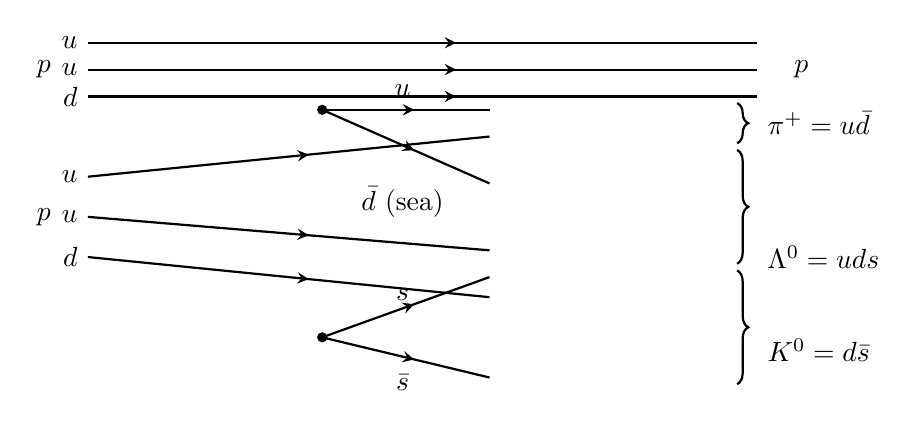
\begin{tikzpicture}[thick, scale=0.85, >=stealth]
  % top proton (spectator)
  \draw[->-] (-5,2.6) -- (5,2.6); \node[left] at (-5,2.6){$u$};
  \draw[->-] (-5,2.2) -- (5,2.2); \node[left] at (-5,2.2){$u$};
  \draw[->-] (-5,1.8) -- (5,1.8); \node[left] at (-5,1.8){$d$};
  \node[left] at (-5.4,2.2) {$p$};
  \node[right] at (5.4,2.2) {$p$};
  % bottom proton -> Lambda + K0 + pi+
  \draw[->-] (-5,0.6) -- (1.0,1.2); \node[left] at (-5,0.6){$u$};
  \draw[->-] (-5,0.0) -- (1.0,-0.5); \node[left] at (-5,0.0){$u$};
  \draw[->-] (-5,-0.6) -- (1.0,-1.2); \node[left] at (-5,-0.6){$d$};
  \node[left] at (-5.4,0.0) {$p$};
  % sea s sbar
  \node[circle,fill,inner sep=1.3pt] at (-1.5,-1.8) {};
  \draw[->-] (-1.5,-1.8) -- (1.0,-0.9); \node[above] at (-0.3,-1.4){$s$};
  \draw[->-] (-1.5,-1.8) -- (1.0,-2.4); \node[below] at (-0.3,-2.2){$\bar s$};
  % sea u ubar (for pi+)
  \node[circle,fill,inner sep=1.3pt] at (-1.5,1.6) {};
  \draw[->-] (-1.5,1.6) -- (1.0,1.6); \node[above] at (-0.3,1.65){$u$};
  \draw[->-] (-1.5,1.6) -- (1.0,0.5); \node[below] at (-0.3,0.6){$\bar d$ (sea)};
  % grouping labels
  \node[right] at (5.0,1.4) {$\pi^+ = u\bar d$};
  \node[right] at (5.0,-0.6) {$\Lambda^0 = uds$};
  \node[right] at (5.0,-2.0) {$\Kz = d\bar s$};
  % bracket lines
  \draw[decorate, decoration={brace, amplitude=4pt}] (4.7,1.7) -- (4.7,1.1);
  \draw[decorate, decoration={brace, amplitude=4pt}] (4.7,1.0) -- (4.7,-0.7);
  \draw[decorate, decoration={brace, amplitude=4pt}] (4.7,-0.8) -- (4.7,-2.5);
\end{tikzpicture}
\end{center}

\textbf{Regeneration.} After many $\tau_S$ in vacuum:
\[ |\psi\rangle = |K^0_L\rangle = \tfrac{1}{\sqrt 2}\bigl(|\Kz\rangle - |\Kbar\rangle\bigr). \]
Through matter, forward amplitudes differ ($\Kbar N\to \Lambda\pi$ is open, $\Kz N$ is not):
\[ |\psi\rangle_{\text{out}} = \tfrac{1}{\sqrt 2}\bigl(f|\Kz\rangle - \bar f|\Kbar\rangle\bigr). \]
Re-express in $K_S, K_L$:
\[ \boxed{\;|\psi\rangle_{\text{out}} = \tfrac{f-\bar f}{2}|K^0_S\rangle + \tfrac{f+\bar f}{2}|K^0_L\rangle.\;} \]
$K_S$ component is regenerated (Pais--Piccioni).

\subsection*{(d)}

Mass eigenstate: well-defined mass $m_S$ and width $\Gamma_S = 1/\tau_S$. Stationary part: $e^{-i m_S t}$. Decay of $|A|^2\propto e^{-t/\tau_S}$ requires:
\[ \boxed{\;A_S(t) = A_S(0)\,e^{-i m_S t}\,e^{-t/(2\tau_S)},\qquad A_L(t) = A_L(0)\,e^{-i m_L t}\,e^{-t/(2\tau_L)}.\;} \]
Equivalent to complex energy $E_{S,L} = m_{S,L} - i\Gamma_{S,L}/2$ (Wigner--Weisskopf).

In $CP$-conserving limit $K^0_S = |+\rangle$, $K^0_L = |-\rangle$:
\[ |\Kz\rangle = \tfrac{1}{\sqrt2}(|K^0_S\rangle + |K^0_L\rangle),\qquad |\Kbar\rangle = \tfrac{1}{\sqrt2}(|K^0_S\rangle - |K^0_L\rangle). \]
Project:
\[ \boxed{\;A_{\Kz}(t) = \tfrac{1}{\sqrt 2}\bigl(A_S(t) + A_L(t)\bigr),\qquad A_{\Kbar}(t) = \tfrac{1}{\sqrt 2}\bigl(A_S(t) - A_L(t)\bigr).\;} \]

\subsection*{(e)}

Initial $|\psi(0)\rangle=|\Kz\rangle$: $A_S(0)=A_L(0)=1/\sqrt 2$.

Substitute into part (d):
\[ A_{\Kz}(t) = \tfrac{1}{2}\bigl(e^{-im_S t}e^{-t/(2\tau_S)} + e^{-im_L t}e^{-t/(2\tau_L)}\bigr). \]
\[ A_{\Kbar}(t) = \tfrac{1}{2}\bigl(e^{-im_S t}e^{-t/(2\tau_S)} - e^{-im_L t}e^{-t/(2\tau_L)}\bigr). \]
Square modulus:
\[ |A_{\Kz}|^2 = \tfrac{1}{4}\bigl(e^{-t/\tau_S} + e^{-t/\tau_L} + 2 e^{-t/(2\tau_S)}e^{-t/(2\tau_L)}\cos[(m_L-m_S)t]\bigr). \]
\[ |A_{\Kbar}|^2 = \tfrac{1}{4}\bigl(e^{-t/\tau_S} + e^{-t/\tau_L} - 2 e^{-t/(2\tau_S)}e^{-t/(2\tau_L)}\cos[(m_L-m_S)t]\bigr). \]
Match to $I = A e^{-t/\tau_S} + B e^{-t/\tau_L} + C\cos\phi$:
\[ \boxed{\;A = B = \tfrac14,\quad C = \pm \tfrac12 e^{-t/(2\tau_S)} e^{-t/(2\tau_L)},\quad \phi = \Delta m\, t,\;} \]
$+$ for $\Kz$, $-$ for $\Kbar$, $\Delta m = m_L - m_S = 3.49\times 10^{-12}$ MeV/$c^2$.

\textbf{Numerical scales for sketch.} In $\tilde t = t/\tau_S$:
\[ \tau_S/\tau_L = 8.958\times 10^{-11}/5.18\times 10^{-8} = 1.73\times 10^{-3}. \]
\[ \Delta m \,\tau_S /\hbar = (3.49\times 10^{-12}\text{ MeV})(8.958\times 10^{-11}\text{ s})/(6.582\times 10^{-22}\text{ MeV s}). \]
\[ \Delta m \,\tau_S /\hbar \approx 0.475\text{ rad}. \]

\begin{center}
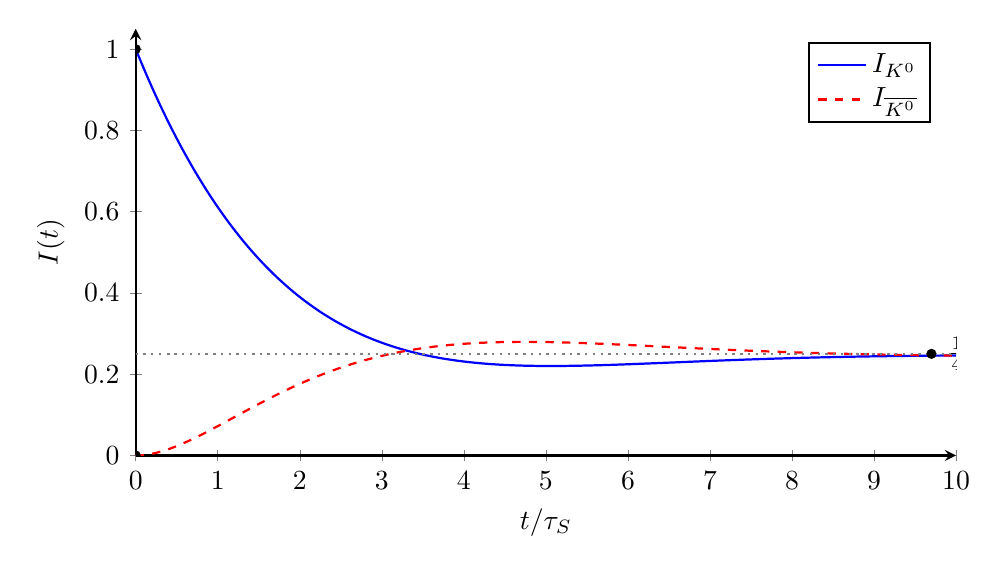
\begin{tikzpicture}
\begin{axis}[
  width=12cm, height=7cm,
  xlabel={$t/\tau_S$}, ylabel={$I(t)$},
  xmin=0, xmax=10, ymin=0, ymax=1.05,
  domain=0:10, samples=300,
  legend pos=north east, thick, axis lines=left,
]
\addplot[blue, thick] {0.25*exp(-x) + 0.25*exp(-1.73e-3*x) + 0.5*exp(-0.5*x)*exp(-0.5*1.73e-3*x)*cos(deg(0.475*x))};
\addlegendentry{$I_{\Kz}$}
\addplot[red, thick, dashed] {0.25*exp(-x) + 0.25*exp(-1.73e-3*x) - 0.5*exp(-0.5*x)*exp(-0.5*1.73e-3*x)*cos(deg(0.475*x))};
\addlegendentry{$I_{\Kbar}$}
\addplot[gray, dotted] {0.25};
\node[circle,fill,inner sep=1.3pt,label={left:$1$}] at (axis cs:0,1) {};
\node[circle,fill,inner sep=1.3pt,label={left:$0$}] at (axis cs:0,0) {};
\node[circle,fill,inner sep=1.3pt,label={right:$\tfrac14$ floor}] at (axis cs:9.7,0.25) {};
\end{axis}
\end{tikzpicture}
\end{center}

%==========================================================
\section*{Question 2 --- Fermi's Golden Rule and Feynman diagrams}

\textbf{Problem.} (a) Define terms in $\Gamma=(2\pi/\hbar)|M|^2\rho$. (b) Diagram and phase-space estimate for $\pi^+\to\mu^+\nu_\mu\gamma$. (c) Estimate $\tau_\tau$ from $\tau_\mu$. (d) Relate diagrams to FGR. (e) Diagrams for Compton, bremsstrahlung, pair production. (f) Diagrams and cross-section ordering for four $e\nu$ channels. (g) Is $\mu^-\to e^-e^-e^+\nu_\mu\bar\nu_e$ allowed?

\subsection*{(a)}

\[ \Gamma = \frac{2\pi}{\hbar}|M|^2 \rho. \]
\begin{itemize}
\item $\Gamma$: transition rate from $|i\rangle$ to continuum of $|f\rangle$ ($=1/\tau$).
\item $M = \langle f | H'|i\rangle$: matrix element of perturbing Hamiltonian.
\item $\rho = \de n / \de E_f$: density of final states at the conserved energy.
\end{itemize}
Validity: $|M|^2 t/\hbar \ll 1$ and $\rho$ smooth (continuum).

\subsection*{(b)}

$\pi^+ \to \mu^+\nu_\mu\gamma$: photon radiated off $\mu^+$ (or pion / $W$):

\begin{center}
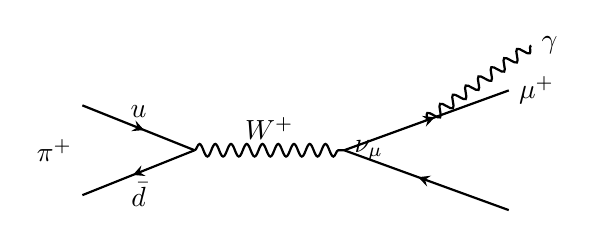
\begin{tikzpicture}[thick, scale=0.95, >=stealth]
  \draw[->-] (-4,0.6) -- (-2.5,0) node[midway, above]{$u$};
  \draw[->-] (-2.5,0) -- (-4,-0.6) node[midway,below]{$\bar d$};
  \node[left] at (-4.0,0) {$\pi^+$};
  \draw[decorate, decoration={snake, amplitude=0.8mm, segment length=2mm}] (-2.5,0) -- (-0.5,0) node[midway,above]{$W^+$};
  \draw[->-] (-0.5,0) -- (1.7,0.8) node[right]{$\mu^+$};
  \draw[->-] (1.7,-0.8) -- (-0.5,0) node[right]{$\nu_\mu$};
  \draw[decorate, decoration={snake, amplitude=0.7mm, segment length=2mm}] (0.6,0.4) -- (2.0,1.4) node[right]{$\gamma$};
\end{tikzpicture}
\end{center}

\textbf{Branching-ratio scaling.} Two-body decay $\pi^+\to\mu^+\nu_\mu$ is helicity-suppressed:
\[ \Gamma_{2} \propto G_F^2 f_\pi^2\, m_\pi\, m_\mu^2 \bigl(1 - m_\mu^2/m_\pi^2\bigr)^2. \]
Photon emission removes the chirality flip; cost is $\alpha$ and three-body phase space.

Two-body phase space:
\[ \Phi_2 \sim \frac{1}{8\pi}. \]
Three-body phase space (relativistic, masses small):
\[ \Phi_3 \sim \frac{m_\pi^2}{192\pi^3}. \]
Form ratio:
\[ \frac{\Gamma(\pi^+\to\mu^+\nu_\mu\gamma)}{\Gamma(\pi^+\to\mu^+\nu_\mu)} \sim \alpha \cdot \frac{1}{m_\mu^2}\cdot \frac{\Phi_3}{\Phi_2}. \]
\[ \boxed{\;\text{BR} \sim \alpha\,\frac{m_\pi^2}{m_\mu^2}\bigl(1-m_\mu^2/m_\pi^2\bigr)^{-2}\times \mathcal{O}(1).\;} \]
Numerical with $\alpha = 1/137$, $m_\pi/m_\mu = 1.32$: BR $\sim 10^{-4}$ (measured: $2\times 10^{-4}$).

Assumptions: same $V-A$ Hamiltonian, universal QED coupling, helicity flip removed, slowly varying form factors.

\subsection*{(c)}

Both purely leptonic weak: $\Gamma\propto G_F^2 m^5/(192\pi^3)$.

Tau has multiple open channels:
\[ N_{\text{open}} = 1\,(e\bar\nu_e\nu_\tau) + 1\,(\mu\bar\nu_\mu\nu_\tau) + N_c\,(d\bar u, s\bar u) \approx 1+1+3 = 5. \]
Form ratio:
\[ \frac{\tau_\tau}{\tau_\mu} = \frac{1}{N_{\text{open}}}\Big(\frac{m_\mu}{m_\tau}\Big)^5. \]
Numerical with $m_\mu = 105.7$, $m_\tau = 1777$ MeV:
\[ m_\mu/m_\tau = 0.0595. \]
\[ (m_\mu/m_\tau)^5 = 7.4\times 10^{-7}. \]
\[ \tau_\tau = (2.2\times 10^{-6}\text{ s})\times \frac{7.4\times 10^{-7}}{5}. \]
\[ \boxed{\;\tau_\tau \approx 3.3\times 10^{-13}\text{ s}.\;} \]
(Measured: $2.9\times 10^{-13}$ s; QCD enhances $N_{\text{open}}\to\sim 5.6$.)

\subsection*{(d)}

$M$ in FGR is the sum of Feynman amplitudes. Components:
\begin{itemize}
\item \textbf{External lines}: physical incoming/outgoing particles, on-shell.
\item \textbf{Propagators (internal lines)}: virtual quanta, factor $i/(p^2-m^2+i\epsilon)$.
\item \textbf{Vertices}: coupling $\times$ Dirac structure (e.g.\ $-ie\gamma^\mu$ for QED); enforce 4-momentum conservation.
\item \textbf{Loops}: $\int \de^4 k/(2\pi)^4$.
\end{itemize}
Square, average over initial spins, sum over final spins, fold in $\rho$ $\Rightarrow$ $\Gamma$.

\subsection*{(e)}

\begin{center}
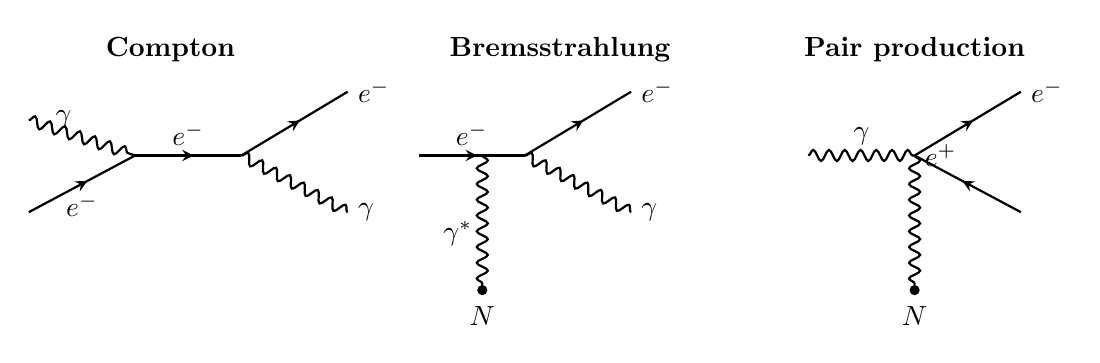
\begin{tikzpicture}[thick, scale=0.9, >=stealth]
  \node at (-5.0,2.0){\textbf{Compton}};
  \draw[decorate, decoration={snake, amplitude=0.7mm, segment length=2mm}] (-7,1) -- (-5.5,0.5) node[midway,above left]{$\gamma$};
  \draw[->-] (-7,-0.3) -- (-5.5,0.5) node[midway, below]{$e^-$};
  \draw[->-] (-5.5,0.5) -- (-4.0,0.5) node[midway,above]{$e^-$};
  \draw[->-] (-4.0,0.5) -- (-2.5,1.4) node[right]{$e^-$};
  \draw[decorate, decoration={snake, amplitude=0.7mm, segment length=2mm}] (-4.0,0.5) -- (-2.5,-0.3) node[right]{$\gamma$};
  %
  \node at (0.5,2.0){\textbf{Bremsstrahlung}};
  \draw[->-] (-1.5,0.5) -- (0,0.5) node[midway,above]{$e^-$};
  \draw[->-] (0,0.5) -- (1.5,1.4) node[right]{$e^-$};
  \draw[decorate, decoration={snake, amplitude=0.7mm, segment length=2mm}] (0,0.5) -- (1.5,-0.3) node[right]{$\gamma$};
  \draw[decorate, decoration={snake, amplitude=0.7mm, segment length=2mm}] (-0.6,0.5) -- (-0.6,-1.4);
  \node[left] at (-0.6,-0.6) {$\gamma^*$};
  \node[circle,fill,inner sep=1.3pt,label=below:{$N$}] at (-0.6,-1.4) {};
  %
  \node at (5.5,2.0){\textbf{Pair production}};
  \draw[decorate, decoration={snake, amplitude=0.7mm, segment length=2mm}] (4,0.5) -- (5.5,0.5) node[midway,above]{$\gamma$};
  \draw[->-] (5.5,0.5) -- (7,1.4) node[right]{$e^-$};
  \draw[->-] (7,-0.3) -- (5.5,0.5) node[right]{$e^+$};
  \draw[decorate, decoration={snake, amplitude=0.7mm, segment length=2mm}] (5.5,0.5) -- (5.5,-1.4);
  \node[circle,fill,inner sep=1.3pt,label=below:{$N$}] at (5.5,-1.4) {};
\end{tikzpicture}
\end{center}

\subsection*{(f)}

\begin{center}
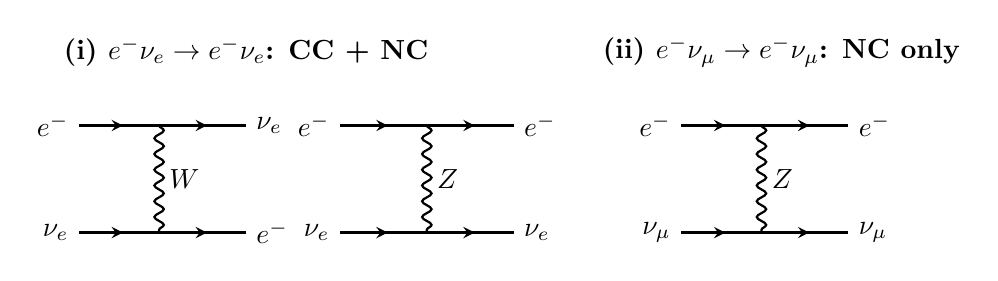
\begin{tikzpicture}[thick, scale=0.85, >=stealth]
  % (i)
  \node at (-5.0,2.4) {\textbf{(i) $e^-\nu_e\to e^-\nu_e$: CC + NC}};
  \draw[->-] (-7.5,1.3) -- (-6.3,1.3); \node[left] at (-7.5,1.3){$e^-$};
  \draw[->-] (-6.3,1.3) -- (-5.0,1.3); \node[right] at (-5.0,1.3){$\nu_e$};
  \draw[->-] (-7.5,-0.3) -- (-6.3,-0.3); \node[left] at (-7.5,-0.3){$\nu_e$};
  \draw[->-] (-6.3,-0.3) -- (-5.0,-0.3); \node[right] at (-5.0,-0.3){$e^-$};
  \draw[decorate, decoration={snake, amplitude=0.6mm, segment length=2mm}] (-6.3,1.3) -- (-6.3,-0.3); \node[right] at (-6.3,0.5){$W$};
  %
  \draw[->-] (-3.6,1.3) -- (-2.3,1.3); \node[left] at (-3.6,1.3){$e^-$};
  \draw[->-] (-2.3,1.3) -- (-1.0,1.3); \node[right] at (-1.0,1.3){$e^-$};
  \draw[->-] (-3.6,-0.3) -- (-2.3,-0.3); \node[left] at (-3.6,-0.3){$\nu_e$};
  \draw[->-] (-2.3,-0.3) -- (-1.0,-0.3); \node[right] at (-1.0,-0.3){$\nu_e$};
  \draw[decorate, decoration={snake, amplitude=0.6mm, segment length=2mm}] (-2.3,1.3) -- (-2.3,-0.3); \node[right] at (-2.3,0.5){$Z$};
  %
  \node at (3.0,2.4) {\textbf{(ii) $e^-\nu_\mu\to e^-\nu_\mu$: NC only}};
  \draw[->-] (1.5,1.3) -- (2.7,1.3); \node[left] at (1.5,1.3){$e^-$};
  \draw[->-] (2.7,1.3) -- (4.0,1.3); \node[right] at (4.0,1.3){$e^-$};
  \draw[->-] (1.5,-0.3) -- (2.7,-0.3); \node[left] at (1.5,-0.3){$\nu_\mu$};
  \draw[->-] (2.7,-0.3) -- (4.0,-0.3); \node[right] at (4.0,-0.3){$\nu_\mu$};
  \draw[decorate, decoration={snake, amplitude=0.6mm, segment length=2mm}] (2.7,1.3) -- (2.7,-0.3); \node[right] at (2.7,0.5){$Z$};
\end{tikzpicture}

\vspace{4pt}

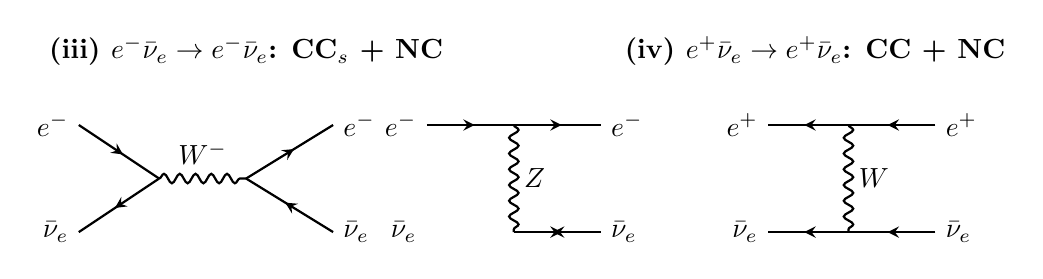
\begin{tikzpicture}[thick, scale=0.85, >=stealth]
  \node at (-5.0,2.4) {\textbf{(iii) $e^-\bar\nu_e\to e^-\bar\nu_e$: CC$_s$ + NC}};
  \draw[->-] (-7.5,1.3) -- (-6.3,0.5); \node[left] at (-7.5,1.3){$e^-$};
  \draw[->-] (-6.3,0.5) -- (-7.5,-0.3); \node[left] at (-7.5,-0.3){$\bar\nu_e$};
  \draw[decorate, decoration={snake, amplitude=0.6mm, segment length=2mm}] (-6.3,0.5) -- (-5.0,0.5); \node[above] at (-5.65,0.55){$W^-$};
  \draw[->-] (-5.0,0.5) -- (-3.7,1.3); \node[right] at (-3.7,1.3){$e^-$};
  \draw[->-] (-3.7,-0.3) -- (-5.0,0.5); \node[right] at (-3.7,-0.3){$\bar\nu_e$};
  %
  \draw[->-] (-2.3,1.3) -- (-1.0,1.3); \node[left] at (-2.3,1.3){$e^-$};
  \draw[->-] (-1.0,1.3) -- (0.3,1.3); \node[right] at (0.3,1.3){$e^-$};
  \draw[->-] (0.3,-0.3) -- (-1.0,-0.3); \node[left] at (-2.3,-0.3){$\bar\nu_e$};
  \draw[->-] (-1.0,-0.3) -- (0.3,-0.3); \node[right] at (0.3,-0.3){$\bar\nu_e$};
  \draw[decorate, decoration={snake, amplitude=0.6mm, segment length=2mm}] (-1.0,1.3) -- (-1.0,-0.3); \node[right] at (-1.0,0.5){$Z$};
  %
  \node at (3.5,2.4) {\textbf{(iv) $e^+\bar\nu_e\to e^+\bar\nu_e$: CC + NC}};
  \draw[->-] (4.0,1.3) -- (2.8,1.3); \node[left] at (2.8,1.3){$e^+$};
  \draw[->-] (5.3,1.3) -- (4.0,1.3); \node[right] at (5.3,1.3){$e^+$};
  \draw[->-] (4.0,-0.3) -- (2.8,-0.3); \node[left] at (2.8,-0.3){$\bar\nu_e$};
  \draw[->-] (5.3,-0.3) -- (4.0,-0.3); \node[right] at (5.3,-0.3){$\bar\nu_e$};
  \draw[decorate, decoration={snake, amplitude=0.6mm, segment length=2mm}] (4.0,1.3) -- (4.0,-0.3); \node[right] at (4.0,0.5){$W$};
\end{tikzpicture}
\end{center}

All weak: $\sigma\propto G_F^2 s$ at $\sqrt s\ll M_W$. Channels available:
\begin{itemize}
\item (i) CC + NC, constructive interference $\Rightarrow$ largest.
\item (ii) NC only $\Rightarrow$ smallest.
\item (iii) CC s-channel + NC.
\item (iv) CC + NC, different chirality structure than (i).
\end{itemize}
\[ \boxed{\;\sigma_{(\text{i})} > \sigma_{(\text{iv})} > \sigma_{(\text{iii})} > \sigma_{(\text{ii})}.\;} \]

\subsection*{(g)}

Process $\mu^-\to e^-e^-e^+\nu_\mu\bar\nu_e$. Quantum numbers:
\[ Q: -1 \to -1-1+1+0+0 = -1.\;\checkmark \]
\[ L_\mu: +1 \to +1.\;\checkmark \]
\[ L_e: 0 \to (+1)+(+1)+(-1)+(-1) = 0.\;\checkmark \]
\textbf{Allowed.} It is ordinary muon decay with an extra internal $\gamma^*\to e^+e^-$:

\begin{center}
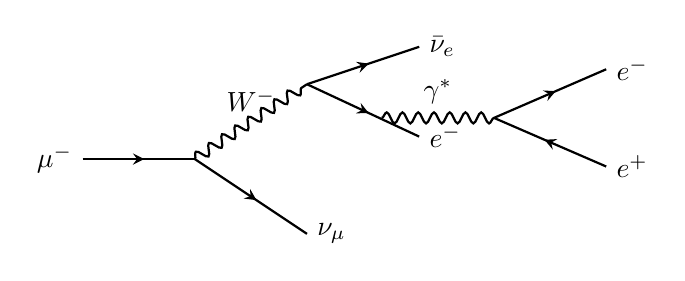
\begin{tikzpicture}[thick, scale=0.95, >=stealth]
  \draw[->-] (-5,0) -- (-3.5,0); \node[left] at (-5,0){$\mu^-$};
  \draw[decorate, decoration={snake, amplitude=0.7mm, segment length=2mm}] (-3.5,0) -- (-2,1); \node[above] at (-2.75,0.5){$W^-$};
  \draw[->-] (-3.5,0) -- (-2,-1); \node[right] at (-2,-1){$\nu_\mu$};
  \draw[->-] (-2,1) -- (-0.5,1.5); \node[right] at (-0.5,1.5){$\bar\nu_e$};
  \draw[->-] (-2,1) -- (-0.5,0.3); \node[right] at (-0.5,0.3){$e^-$};
  \draw[decorate, decoration={snake, amplitude=0.7mm, segment length=2mm}] (-1.0,0.55) -- (0.5,0.55); \node[above] at (-0.25,0.6){$\gamma^*$};
  \draw[->-] (0.5,0.55) -- (2,1.2); \node[right] at (2,1.2){$e^-$};
  \draw[->-] (2,-0.1) -- (0.5,0.55); \node[right] at (2,-0.1){$e^+$};
\end{tikzpicture}
\end{center}

BR suppressed by $\alpha^2 \sim 5\times 10^{-5}$ relative to ordinary muon decay.

%==========================================================
\section*{Question 3 --- $\beta$, $\alpha$ decay; chain kinetics}

\textbf{Problem.} (a) $Q$-values for $\beta^\mp$ and EC in atomic masses. (b) $T_\alpha(Q,A)$. (c) Assumptions in Gamow factor. (d) For $a\to b\to c$: (i) $\alpha,\beta$, (ii) $t_{\max}$ when $N_{b0}=0$, (iii) $N_c(t)$.

\subsection*{(a)}

Atomic masses $M(P), M(D)$; nuclear $M_{\text{nuc}}(P) = M(P) - Z m_e$; (anti)$\nu$ massless.

\textbf{$\beta^-$:} ${}^A_Z P\to {}^A_{Z+1} D + e^-+\bar\nu_e$. Nuclear-level energy balance:
\[ Q = M_{\text{nuc}}(P) - M_{\text{nuc}}(D) - m_e. \]
Substitute atomic masses ($Z+1$ electrons on the daughter side absorb the emitted $e^-$):
\[ \boxed{\;Q_{\beta^-} = [M(P) - M(D)]c^2.\;} \]

\textbf{$\beta^+$:} ${}^A_Z P\to {}^A_{Z-1} D + e^++\nu_e$. Nuclear-level:
\[ Q = M_{\text{nuc}}(P) - M_{\text{nuc}}(D) - m_e. \]
Substitute atomic ($D$ has $Z-1$ electrons):
\[ \boxed{\;Q_{\beta^+} = [M(P) - M(D) - 2 m_e]c^2.\;} \]

\textbf{Electron capture:} ${}^A_Z P + e^- \to {}^A_{Z-1} D + \nu_e$. Captured electron is atomic $K$-shell, binding $B_e$:
\[ \boxed{\;Q_{\text{EC}} = [M(P)-M(D)]c^2 - B_e.\;} \]
EC remains open when $\beta^+$ closes (no $2 m_e$ penalty, only $B_e\sim$ keV).

\subsection*{(b)}

${}^A_Z P\to {}^{A-4}_{Z-2} D + \alpha$ at rest. Momentum conservation:
\[ |\vec p_\alpha| = |\vec p_D| \equiv p. \]
Non-relativistic ($Q\ll M_D$):
\[ T_\alpha = \frac{p^2}{2 m_\alpha},\qquad T_D = \frac{p^2}{2 M_D}. \]
Form ratio:
\[ \frac{T_D}{T_\alpha} = \frac{m_\alpha}{M_D}. \]
Substitute into $Q = T_\alpha + T_D$:
\[ T_\alpha = Q\cdot\frac{M_D}{m_\alpha + M_D}. \]
Use $m_\alpha\approx 4 u$, $M_D \approx (A-4) u$:
\[ \boxed{\;T_\alpha = Q\Big(1 - \frac{4}{A}\Big).\;} \]

\subsection*{(c)}

$\tau\propto \exp[Z e^2/(\epsilon_0 \hbar v)]$ from WKB tunnelling of pre-formed $\alpha$ through Coulomb barrier. Assumptions:
\begin{enumerate}
\item Pre-formed $\alpha$ cluster inside parent, assault frequency $\nu_0 \sim v/(2R)$.
\item Daughter as point charge $(Z-2)e$; Coulomb barrier outside $R$ only.
\item Centrifugal barrier neglected (s-wave).
\item WKB: $V-E$ slow on de Broglie scale.
\item Low-velocity limit: inner turning point $\to 0$; leading exponent $Ze^2/(\epsilon_0\hbar v)$.
\item Energy-independent prefactor; all $(Z,v)$-dependence in exponent.
\end{enumerate}
Result: Geiger--Nuttall straight line over $\sim$ 24 decades.

\subsection*{(d)(i)}

Bateman equations:
\[ \frac{\de N_a}{\de t} = -\lambda_a N_a,\qquad \frac{\de N_b}{\de t} = \lambda_a N_a - \lambda_b N_b. \]
Integrate first equation:
\[ N_a(t) = N_{a0}\,e^{-\lambda_a t}. \]
Substitute into second:
\[ \frac{\de N_b}{\de t} + \lambda_b N_b = \lambda_a N_{a0}\,e^{-\lambda_a t}. \]
Multiply by integrating factor $e^{\lambda_b t}$:
\[ \frac{\de}{\de t}\bigl(N_b\,e^{\lambda_b t}\bigr) = \lambda_a N_{a0}\,e^{(\lambda_b - \lambda_a)t}. \]
Integrate:
\[ N_b\,e^{\lambda_b t} = \frac{\lambda_a N_{a0}}{\lambda_b - \lambda_a}\,e^{(\lambda_b-\lambda_a) t} + K. \]
Apply $N_b(0)=N_{b0}$:
\[ K = N_{b0} - \frac{\lambda_a N_{a0}}{\lambda_b - \lambda_a}. \]
Read off coefficients:
\[ \boxed{\;\alpha = \frac{\lambda_a N_{a0}}{\lambda_b - \lambda_a},\qquad \beta = N_{b0} - \frac{\lambda_a N_{a0}}{\lambda_b-\lambda_a}.\;} \]

\subsection*{(d)(ii)}

Set $N_{b0}=0$:
\[ N_b(t) = \frac{\lambda_a N_{a0}}{\lambda_b - \lambda_a}\bigl(e^{-\lambda_a t} - e^{-\lambda_b t}\bigr). \]
Differentiate, set $\de N_b/\de t = 0$:
\[ -\lambda_a e^{-\lambda_a t} + \lambda_b e^{-\lambda_b t} = 0. \]
Rearrange:
\[ e^{(\lambda_b - \lambda_a) t} = \frac{\lambda_b}{\lambda_a}. \]
Solve:
\[ \boxed{\;t_{\max} = \frac{\ln(\lambda_b/\lambda_a)}{\lambda_b - \lambda_a}.\;} \]

\subsection*{(d)(iii)}

$c$ stable: $\de N_c/\de t = \lambda_b N_b$:
\[ \frac{\de N_c}{\de t} = \frac{\lambda_a \lambda_b N_{a0}}{\lambda_b - \lambda_a}\bigl(e^{-\lambda_a t} - e^{-\lambda_b t}\bigr). \]
Integrate from $0$ to $t$ with $N_c(0)=0$:
\[ N_c(t) = \frac{\lambda_a \lambda_b N_{a0}}{\lambda_b - \lambda_a}\Big[\frac{1-e^{-\lambda_a t}}{\lambda_a} - \frac{1-e^{-\lambda_b t}}{\lambda_b}\Big]. \]
Combine over common denominator:
\[ N_c(t) = \frac{N_{a0}}{\lambda_b - \lambda_a}\bigl[\lambda_b(1-e^{-\lambda_a t}) - \lambda_a (1-e^{-\lambda_b t})\bigr]. \]
Simplify:
\[ \boxed{\;N_c(t) = N_{a0}\Big[1 - \frac{\lambda_b\,e^{-\lambda_a t} - \lambda_a\,e^{-\lambda_b t}}{\lambda_b - \lambda_a}\Big].\;} \]
Check: $N_c(0)=0$, $N_c(\infty)=N_{a0}$, $N_a + N_b + N_c = N_{a0}$.

%==========================================================
\section*{Question 4 --- Eightfold way: $J=1/2$ octet, $J=0$ nonet}

\textbf{Problem.} (a) Meaning of $B,S,I_z$; reproduce octet pattern and identify $X',Y'$. (b) One state per edge, none at corners. (c) Two centre states. (d) Evidence for $qqq$. (e) $Q(I_z, S+B)$ relation; quark charges. (f) $\Sigma^0$ decay. (g) $J=0$ meson nonet.

\subsection*{(a)}

\textbf{Definitions:}
\begin{itemize}
\item $B = (n_q - n_{\bar q})/3$: each quark $+1/3$, antiquark $-1/3$.
\item $S = -(n_s - n_{\bar s})$: $s$ has $S=-1$ (sign convention).
\item $I_z$: SU(2) flavour third component; $u: +1/2$, $d: -1/2$, $s: 0$.
\end{itemize}
For $qqq$ from $\{u,d,s\}$: $S+B = 1 - n_s$. Three rows: $n_s=0,1,2$. Within row, $I_z = (n_u - n_d)/2$.

\[ \begin{array}{l|c|c}
\text{State} & \text{Quark content} & (I_z, S+B) \\\hline
p & uud & (+1/2,+1) \\
n & udd & (-1/2,+1) \\
\Sigma^+ & uus & (+1,0) \\
\Sigma^0 & uds & (0,0) \\
\Lambda^0 & uds & (0,0) \\
\Sigma^- & dds & (-1,0) \\
\Xi^0 & uss & (+1/2,-1) \\
\Xi^- & dss & (-1/2,-1)
\end{array} \]
Identify:
\[ \boxed{\;X' = n = udd,\qquad Y' = p = uud.\;} \]

\subsection*{(b)}

Edge positions: two flavours among three, e.g.\ $(I_z,S+B)=(+1,0)$ requires $uus$. Total wavefunction antisymmetric; colour singlet antisymmetric $\Rightarrow$ spin$\otimes$flavour$\otimes$space symmetric. With $S$-wave (spatial symmetric), spin$\otimes$flavour symmetric. For mixed-symmetry flavour ($uus$) and $J=1/2$, exactly one symmetric combination exists $\Rightarrow$ \textbf{one state}.

Corners: $uuu, ddd, sss$ have totally symmetric flavour, requiring totally symmetric spin $\Rightarrow J=3/2$ only (decuplet $\Delta^{++},\Delta^-,\Omega^-$). \textbf{No $J=1/2$ state}.

\subsection*{(c)}

Centre $(0,0)$: flavour $uds$, three distinct flavours admit two independent mixed-symmetry combinations under three-body permutation:
\begin{itemize}
\item $I_{ud}=1$ (symmetric in $ud$): $\Sigma^0$, $m=1192.6$ MeV.
\item $I_{ud}=0$ (antisymmetric in $ud$): $\Lambda^0$, $m=1115.7$ MeV.
\end{itemize}
Different exchange interactions $\Rightarrow$ different masses.

\subsection*{(d)}

Evidence for $qqq$:
\begin{itemize}
\item $B=+1$ conserved (pair production with antibaryon); excludes $q\bar q$.
\item Half-integer spin $J=1/2$: requires odd fermion count.
\item Magnetic moments: SU(6) prediction $\mu_n/\mu_p = -2/3$ confirmed.
\item Deep inelastic scattering: three valence quarks with charges $+2/3,-1/3,-1/3$.
\end{itemize}

\subsection*{(e)}

Inspect table: $Q$ matches $I_z + (S+B)/2$ for every entry.
\[ \boxed{\;Q = I_z + \tfrac12 (S+B)\quad\text{(Gell-Mann--Nishijima)}.\;} \]
Apply to quarks ($B=1/3$ each, $S=-1$ for $s$):
\[ Q_u = +\tfrac12 + \tfrac12\bigl(0 + \tfrac13\bigr) = +\tfrac{2}{3}. \]
\[ Q_d = -\tfrac12 + \tfrac12\bigl(0 + \tfrac13\bigr) = -\tfrac{1}{3}. \]
\[ Q_s = 0 + \tfrac12\bigl(-1 + \tfrac13\bigr) = -\tfrac{1}{3}. \]
\[ \boxed{\;Q_u = +\tfrac{2}{3},\quad Q_d = -\tfrac{1}{3},\quad Q_s = -\tfrac{1}{3}.\;} \]

\subsection*{(f)}

$\Sigma^0$ and $\Lambda^0$ both $uds$, $J^P=\tfrac12^+$: no flavour change. $\Delta m = 76.9$ MeV $< m_{\pi^0}$ so no hadronic mode. Strong/weak forbidden; only EM:
\[ \boxed{\;\Sigma^0 \to \Lambda^0 + \gamma\;\;(\text{M1, }\tau\sim 10^{-19}\text{ s}).\;} \]
$\Sigma^0\to n\pi^0, p\pi^-$ kinematically open as weak decays but the much faster EM mode dominates the lifetime entirely.

\textbf{Photon energy.} Energy/momentum conservation in $\Sigma^0$ rest frame:
\[ E_\gamma + E_\Lambda = m_{\Sigma^0},\qquad |\vec p_\gamma| = |\vec p_\Lambda| = E_\gamma. \]
Use $E_\Lambda^2 = m_\Lambda^2 + E_\gamma^2$:
\[ m_\Lambda^2 + E_\gamma^2 = (m_{\Sigma^0} - E_\gamma)^2. \]
Expand right side:
\[ m_\Lambda^2 + E_\gamma^2 = m_{\Sigma^0}^2 - 2 m_{\Sigma^0} E_\gamma + E_\gamma^2. \]
Cancel $E_\gamma^2$:
\[ \boxed{\;E_\gamma = \frac{m_{\Sigma^0}^2 - m_\Lambda^2}{2 m_{\Sigma^0}}c^2.\;} \]
Numerical:
\[ E_\gamma = \frac{1192.6^2 - 1115.7^2}{2\times 1192.6}\text{ MeV} = \frac{177580}{2385.2}\text{ MeV} \approx 74.4\text{ MeV}. \]

\subsection*{(g)}

Mesons: $q\bar q$, $3\otimes\bar 3 = 8\oplus 1$. For $J=0$ ground-state pseudoscalars:

\[ \begin{array}{l|c|c}
\text{State} & \text{Content} & (I_z,S) \\\hline
K^+ & u\bar s & (+1/2,+1) \\
K^0 & d\bar s & (-1/2,+1) \\
\pi^+ & u\bar d & (+1,0) \\
\pi^0 & \tfrac{1}{\sqrt2}(u\bar u-d\bar d) & (0,0) \\
\eta & \approx \tfrac{1}{\sqrt6}(u\bar u+d\bar d-2 s\bar s) & (0,0) \\
\eta' & \approx \tfrac{1}{\sqrt3}(u\bar u+d\bar d+s\bar s) & (0,0) \\
\pi^- & d\bar u & (-1,0) \\
\Kbar & s\bar d & (+1/2,-1) \\
K^- & s\bar u & (-1/2,-1)
\end{array} \]

\begin{center}
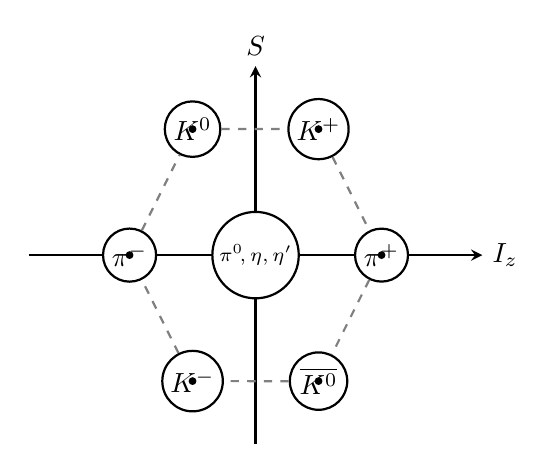
\begin{tikzpicture}[scale=1.6, thick, >=stealth]
  \draw[->] (-1.8,0) -- (1.8,0) node[right]{$I_z$};
  \draw[->] (0,-1.5) -- (0,1.5) node[above]{$S$};
  % top row (S=+1)
  \node[circle,draw,fill=white,inner sep=1.5pt] (Kp) at (0.5,1) {$K^+$};
  \node[circle,draw,fill=white,inner sep=1.5pt] (K0) at (-0.5,1) {$K^0$};
  % middle row (S=0)
  \node[circle,draw,fill=white,inner sep=1.5pt] (pip) at (1.0,0) {$\pi^+$};
  \node[circle,draw,fill=white,inner sep=1.5pt] (pim) at (-1.0,0) {$\pi^-$};
  \node[circle,draw,fill=white,inner sep=1.5pt] (cen) at (0,0) {\scriptsize $\pi^0\!,\eta,\eta'$};
  % bottom row (S=-1)
  \node[circle,draw,fill=white,inner sep=1.5pt] (Kbar) at (0.5,-1) {$\Kbar$};
  \node[circle,draw,fill=white,inner sep=1.5pt] (Km) at (-0.5,-1) {$K^-$};
  % hexagon
  \draw[gray,dashed] (K0) -- (Kp) -- (pip) -- (Kbar) -- (Km) -- (pim) -- (K0);
  % markers
  \node[circle,fill,inner sep=1.0pt] at (0.5,1) {};
  \node[circle,fill,inner sep=1.0pt] at (-0.5,1) {};
  \node[circle,fill,inner sep=1.0pt] at (1.0,0) {};
  \node[circle,fill,inner sep=1.0pt] at (-1.0,0) {};
  \node[circle,fill,inner sep=1.0pt] at (0.5,-1) {};
  \node[circle,fill,inner sep=1.0pt] at (-0.5,-1) {};
\end{tikzpicture}
\end{center}

Pions: $\pi^\pm,\pi^0$. Kaons: $K^\pm, K^0,\Kbar$.

\textbf{Three centre states} ($I_z=0,S=0$), in SU(3) limit:
\begin{itemize}
\item $\pi^0 = \tfrac{1}{\sqrt 2}(u\bar u - d\bar d)$: $I=1$ octet member.
\item $\eta_8 = \tfrac{1}{\sqrt 6}(u\bar u + d\bar d - 2 s\bar s)$: $I=0$ octet member.
\item $\eta_1 = \tfrac{1}{\sqrt 3}(u\bar u + d\bar d + s\bar s)$: SU(3) singlet.
\end{itemize}
SU(3) breaking ($m_s > m_{u,d}$) mixes $\eta_8, \eta_1$ into physical $\eta\,(548)$, $\eta'\,(958)$ MeV. $\pi^0$ is unmixed (different $I$). Anomalously heavy $\eta'$ from U(1)$_A$ axial anomaly.

\end{document}
